%! Author = antonio
%! Date = 7/2/24
The last model we are going to consider is a generative model, the Gaussian Mixture Model (GMM).
This model is based on the assumption that the data is generated by a mixture of K Gaussian distributions.
The GMM density consists of a weighted sum of K Gaussians:

\begin{equation}
    \mathbf{X}\thicksim  GMM(\mathbf{M} ,\mathcal{S},w)\implies f_x(x)=\sum_{c=1}^{K}\mathcal{N}(x|\mu_g,\Sigma_g)w_g
    \label{eq:GMM}
\end{equation}

where \( M=[\mu_1...\mu_k]\), \(\mathcal{S}=[\Sigma_1...\Sigma_k]\) and \(w=[w_1...w_k]\) of \autoref{eq:GMM} are the parameters of the model.\\
Gaussian components can be viewed as clusters to which the samples belong (hard or soft), and the cluster label is an unobserved latent random variable.
We can also define in this case the responsability term, defined as \autoref{eq:responsability}, that represents the
posterior probability that a sample belongs to a certain cluster:

\begin{equation}
    \gamma(z_{n,i})=P(G_i=g| X_i=x)=\frac{f_{x_i,G_i}(x_i,g)}{f_{x_i}(x_i)}=\frac{\mathcal{N}(x_i|\mu_g,\Sigma_g)w_g}{\sum_{g'}\mathcal{N}(x_i|\mu_{g'},\Sigma_{g'})w_{g'}}
    \label{eq:responsability}
\end{equation}

Then assign the sample to the cluster label for which the responsability is highest and re-estimate the model parameters based on the cluster assignment.
We can apply the Expectation-Maximization algorithm to estimate the model parameters.
The EM algorithm is an iterative algorithm that consists of two steps:
\begin{itemize}
    \item Expectation stage: estimation of the responsability (given the model parameters \((M_t,S_t,w_t)\))
    \item Maximization step: estimation of new model parameters using the above statistics, estimation continues from an
    initial value of the model parameters until a certain criterion is met.
\end{itemize}

The EM algorithm then requires an initial estimate for the GMM parameters, so we use the LBG algorithm to incrementally construct a
GMM with 2G components from a GMM with G components.
The starting point will be \( (1,\mu,\sigma)\), so we use the empirical mean and covariance matrix of the data set.
Then it builds a 2-component model starting from one and from each of the new components 2 more components are generated and so on.
GMM can have differents versions as:
\begin{itemize}
    \item \textbf{The full covariance model:} in this case each component has a full covariance matrix, which means that all possible covariances between the variables are considered.
    \item \textbf{The diagonal covariance model:} in this setup, the covariance matrix of each component is assumed to be diagonal, which means the variables are considered independent.
\end{itemize}

As an initial point in our project, we considered having a maximum component number of 32 and using the two methods mentioned above.
So at first we evaluated the model where the number of components for class 0 and class 1 were equal, obtaining the results shown in
\autoref{tab:GMMSameComponents}.
Instead, a graphical view of these results can be seen for the Full Covariance method in \autoref{fig:GMMFullSameComponentF} and
in \autoref{fig:GMMFDiagSameComponentF} for the Diagonal Covariance method.

\begin{figure}[h!]
    \centering
    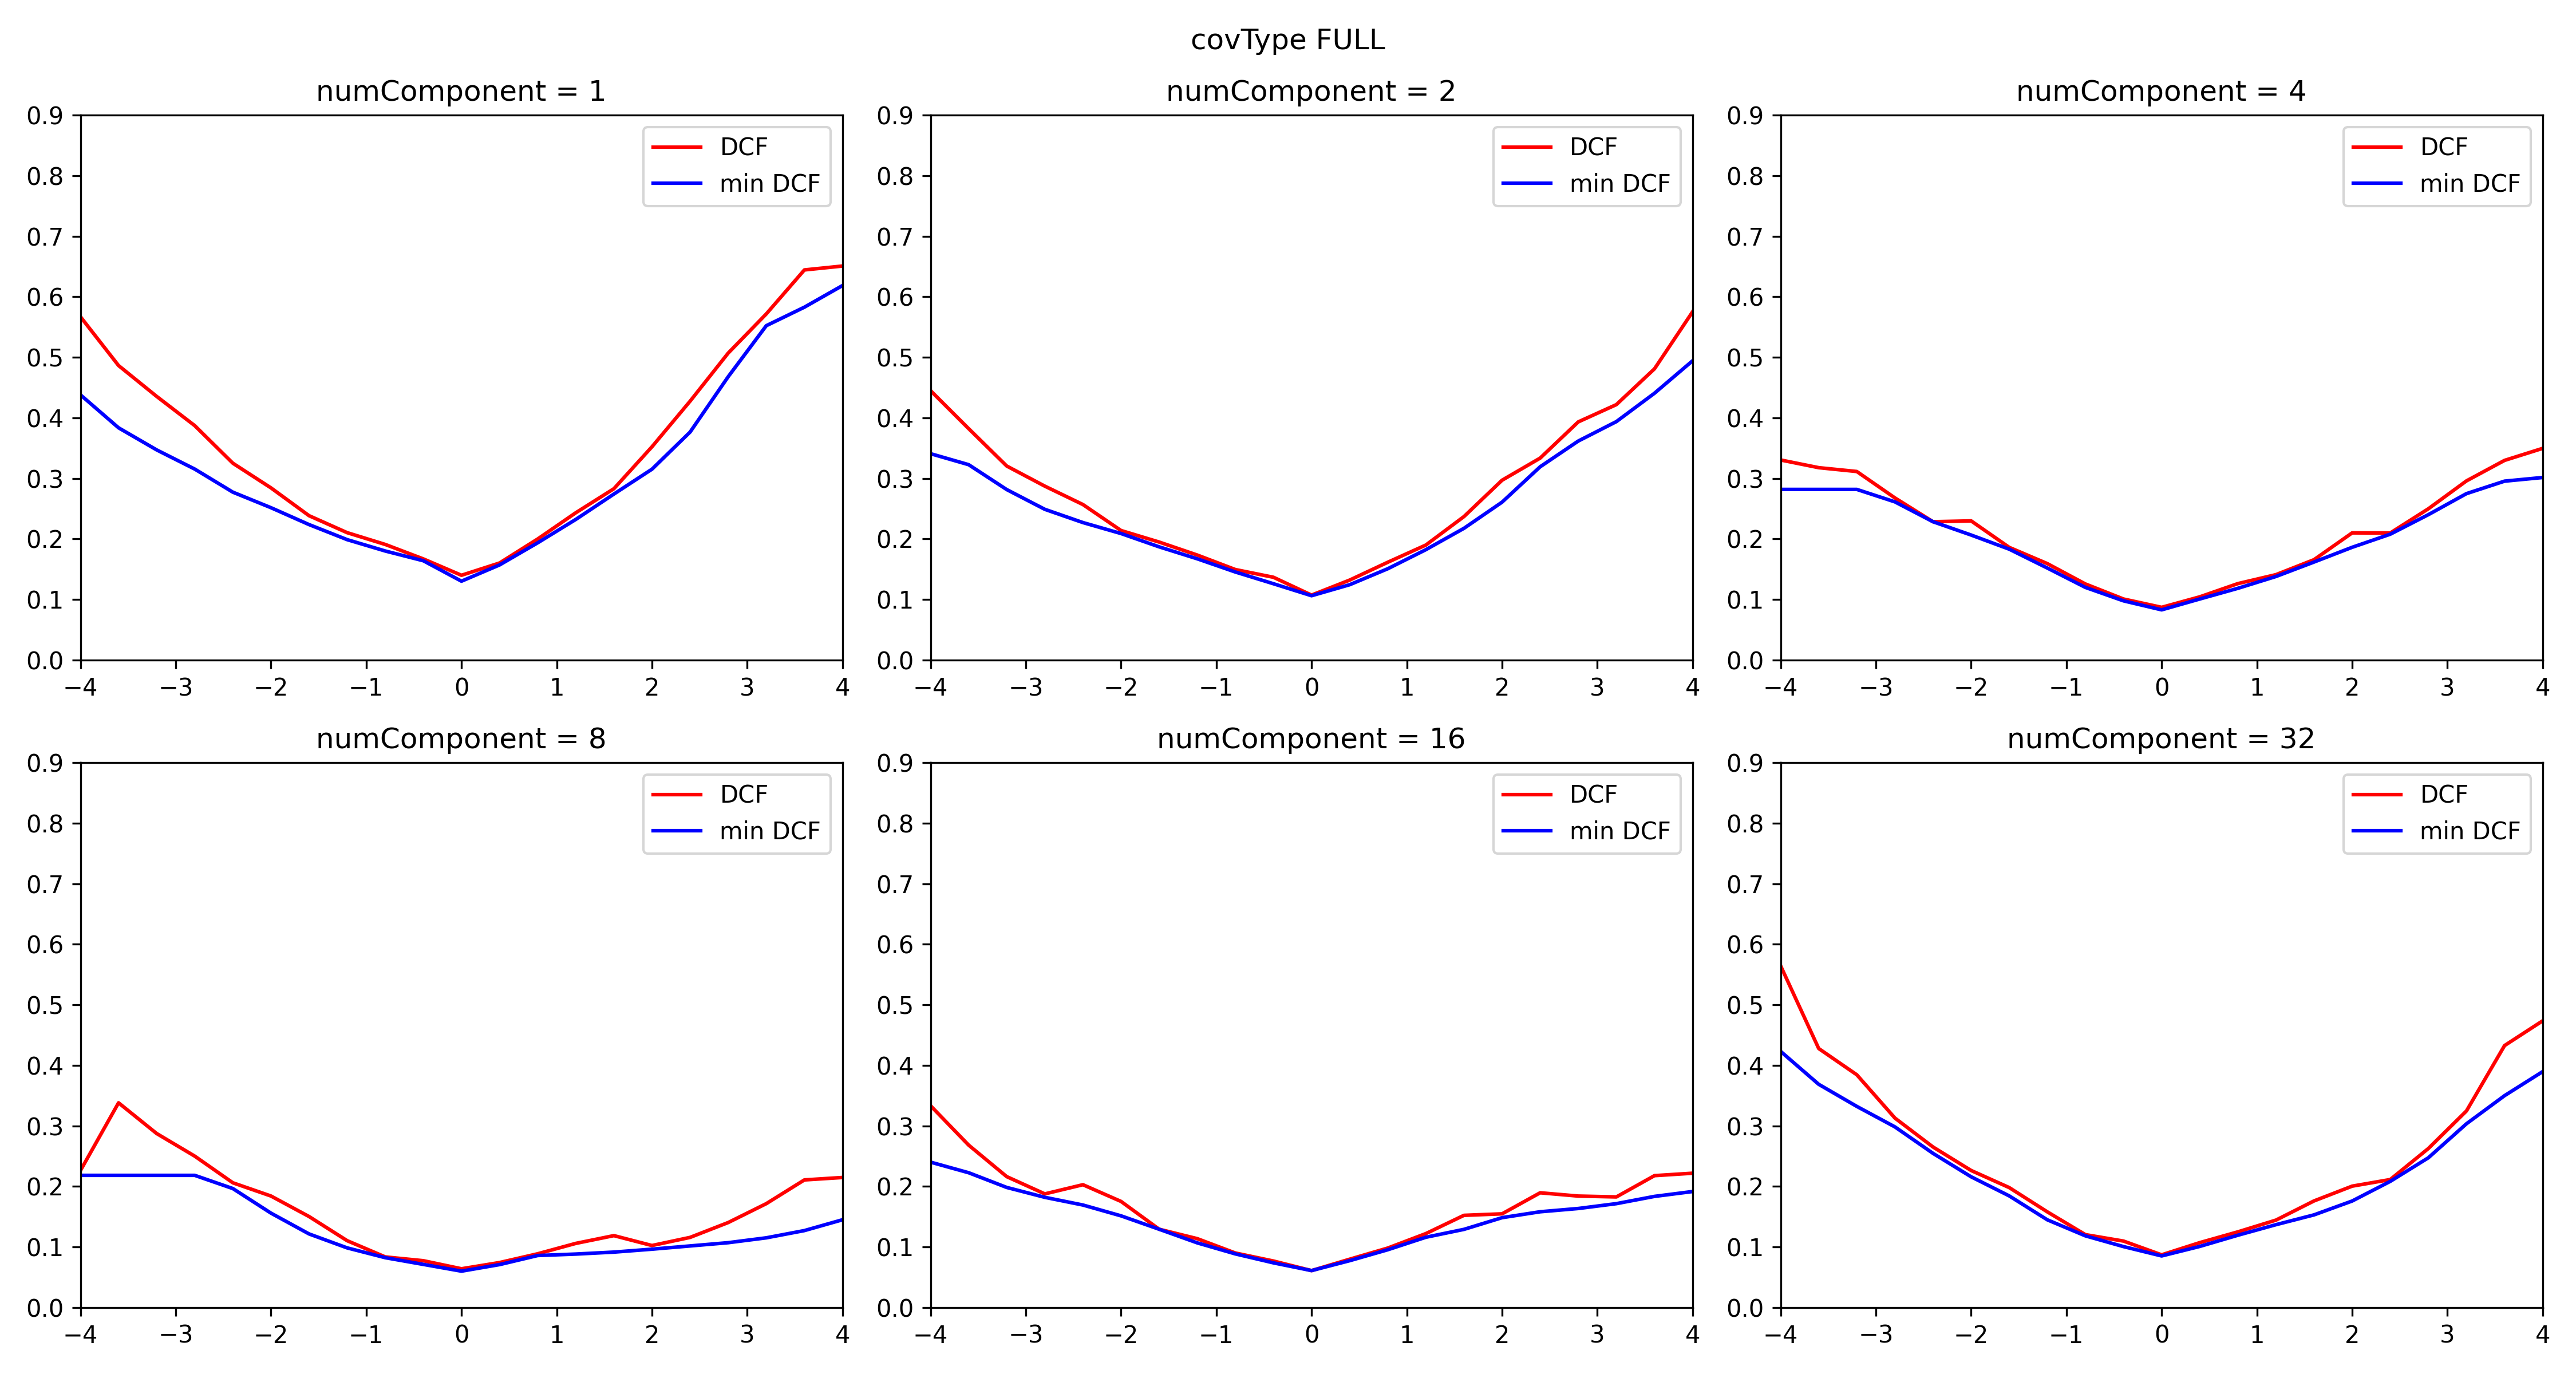
\includegraphics[width=\linewidth]{Lab/10. Lab 10/Images/01. covTypeFullSameComponent}
    \caption{Shows minDCF and actDCF for GMM with Full Covariance and same number of components}
    \label{fig:GMMFullSameComponentF}
\end{figure}

\begin{figure}[h!]
    \centering
    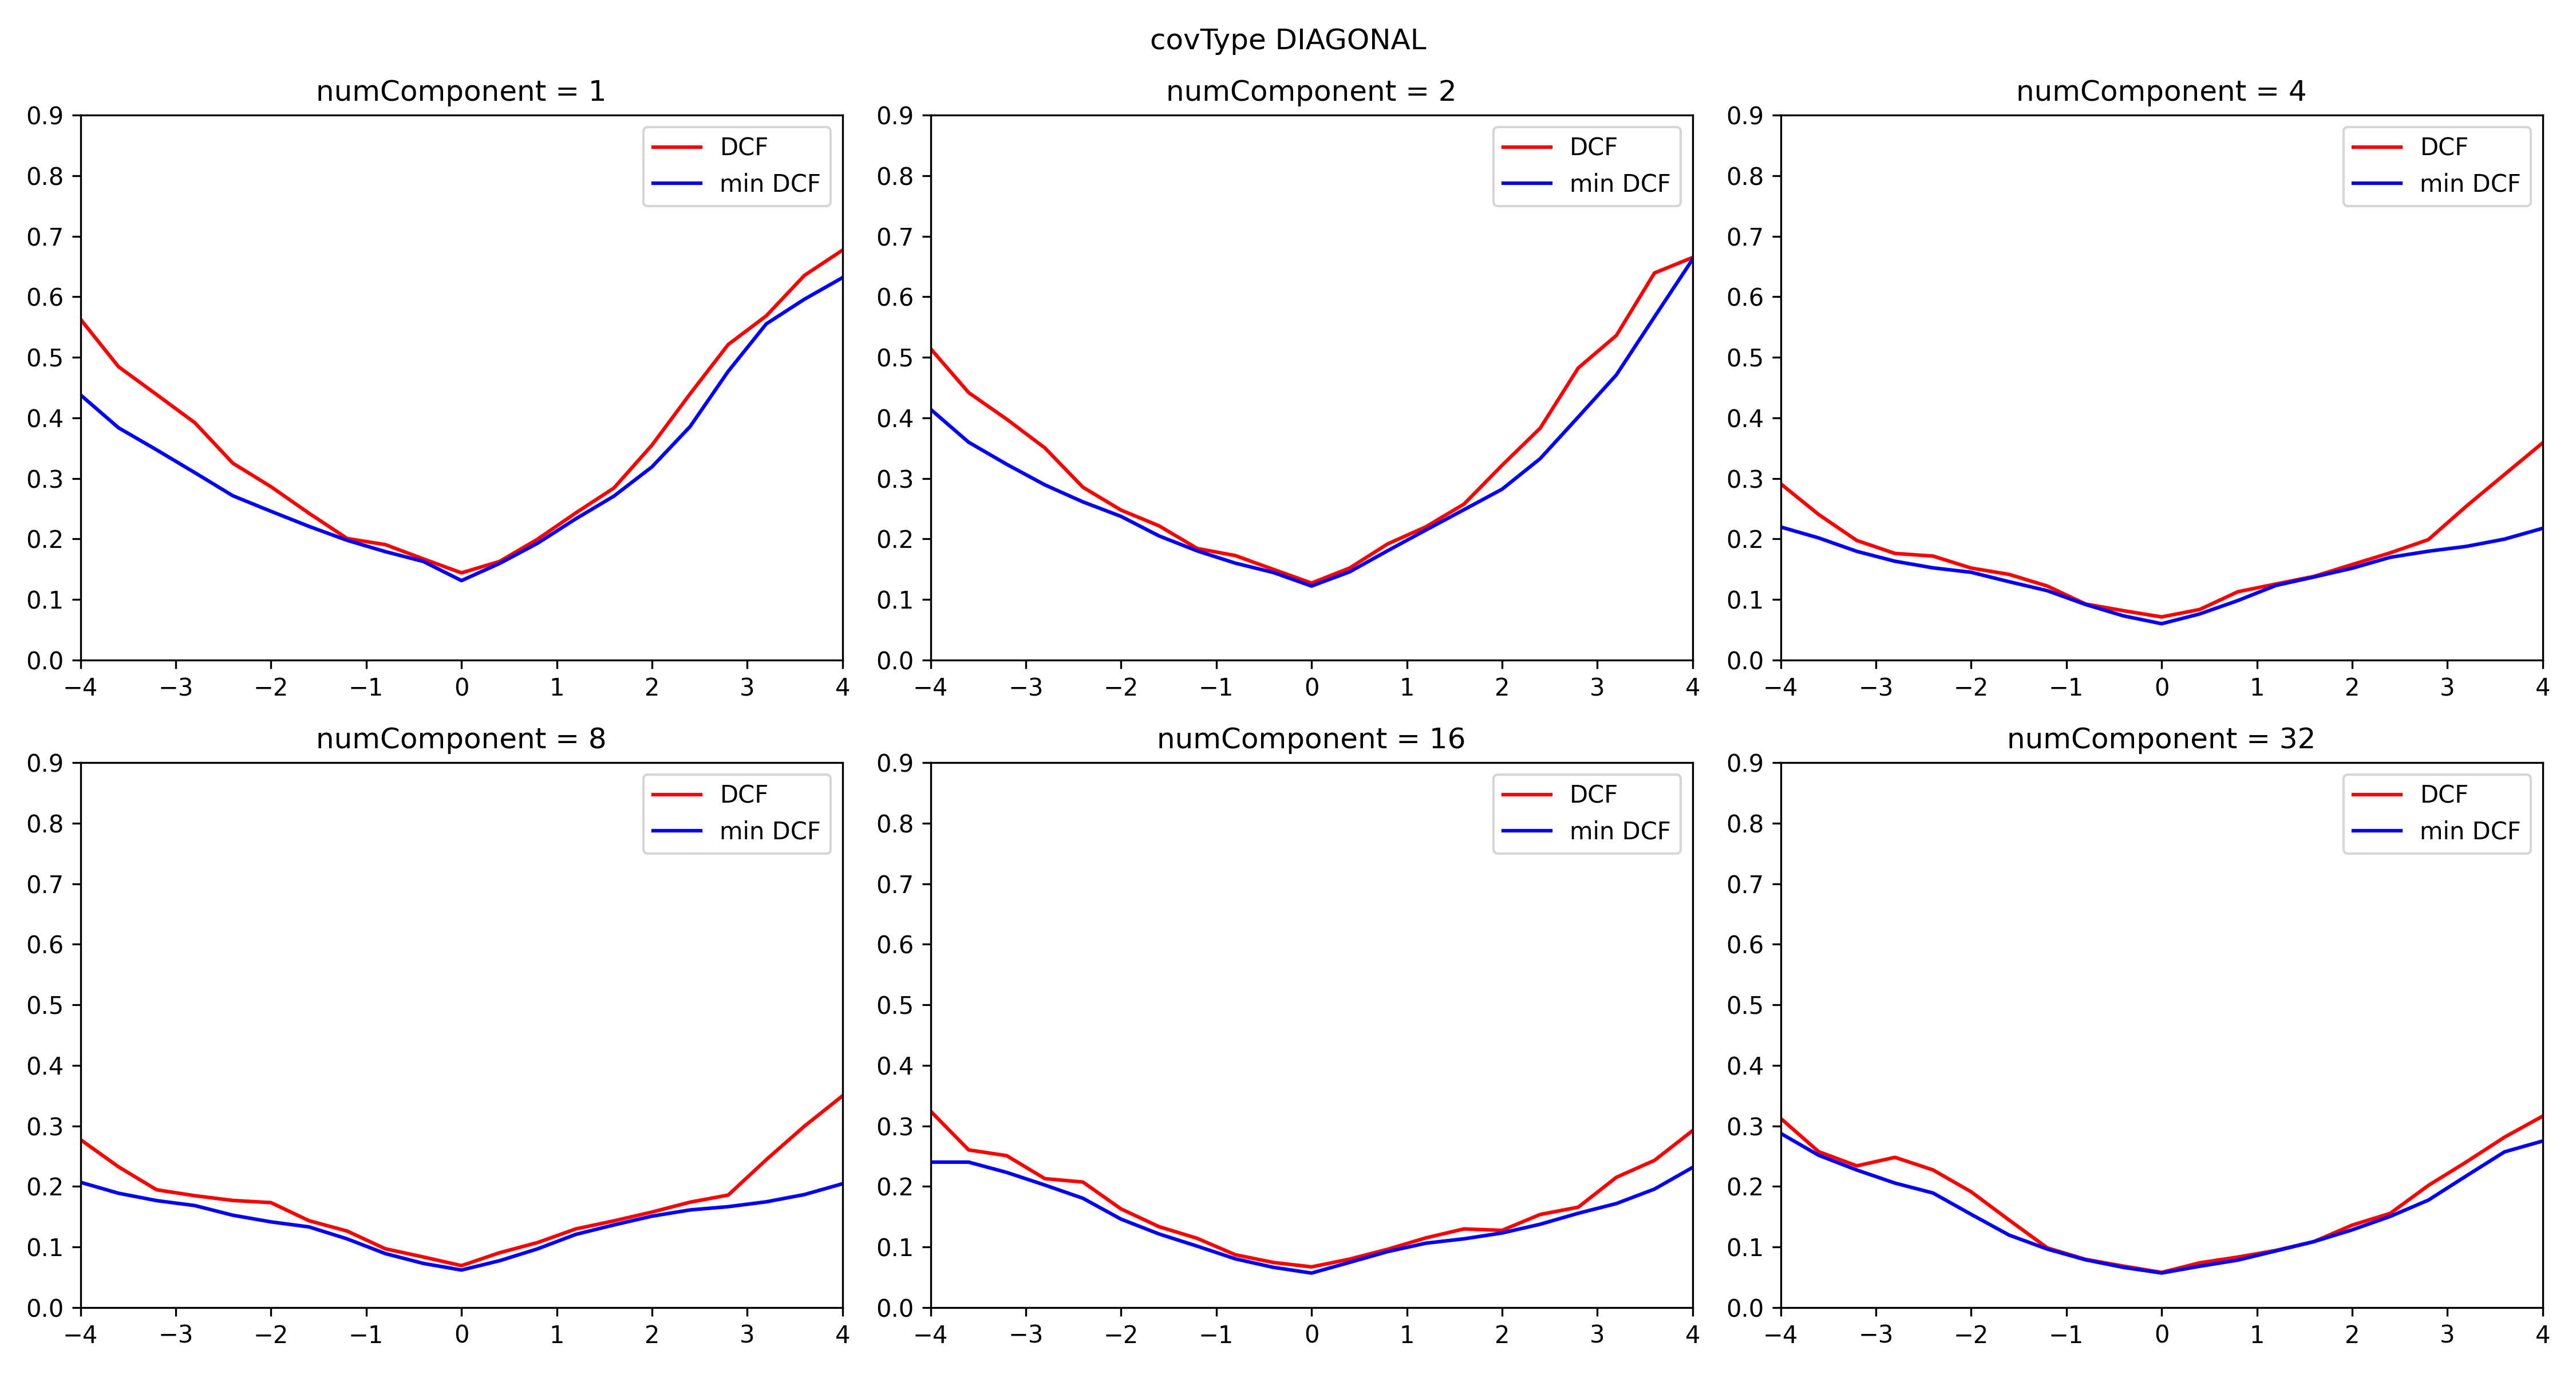
\includegraphics[width=\linewidth]{Lab/10. Lab 10/Images/02. covTypeDiagonalSameComponent}
    \caption{Shows minDCF and actDCF for GMM with Diagonal Covariance and same number of components}
    \label{fig:GMMFDiagSameComponentF}
\end{figure}

\begin{table}[h!]
    \centering
    \begin{tabular}{>{\centering\arraybackslash}p{2cm} >{\centering\arraybackslash}p{2cm} >{\centering\arraybackslash}p{2cm} >{\centering\arraybackslash}p{2cm} >{\centering\arraybackslash}p{2cm}}
        \toprule
        \multicolumn{5}{c}{\textbf{GMM Model}} \\
        \midrule
        \multirow{2}{*}{\textbf{(nc0, nc1)}} & \multicolumn{2}{c}{\textbf{Full Cov}} & \multicolumn{2}{c}{\textbf{Diag Cov}} \\
        \cmidrule(lr){2-5}
        & \textbf{minDCF} & \textbf{actDCF} & \textbf{minDCF} & \textbf{actDCF} \\
        \midrule
        (1, 1)   & 0.2629          & 0.3051          & 0.2570          & 0.3022          \\
        (2, 2)   & 0.2170          & 0.2337          & 0.2489          & 0.2674          \\
        (4, 4)   & 0.2161          & 0.2395          & 0.1481          & 0.1687          \\
        (8, 8)   & 0.1786          & 0.1928          & 0.1463          & 0.1809          \\
        (16, 16) & 0.1631          & 0.1766          & 0.1622          & 0.1769          \\
        (32, 32) & 0.2337          & 0.2499          & 0.1766          & 0.1989          \\
        \bottomrule
    \end{tabular}
    \captionsetup{justification=justified,singlelinecheck=false,format=hang}
    \caption{Show minDCF and actDCF for same number of components in GMM}
    \label{tab:GMMSameComponents}
\end{table}

Subsequently, all possible combinations within the maximum value indicated above were tested.
\autoref{tab:GMMBestComponents} shows what may be the most significant values.
I chose these combinations because (1,16) and (2,16) are the two best combinations for the Full Covariance method,
whereas (8,32) and (8,16) are the best for Diagonal Covariance method.
Their representation is shown in \autoref{fig:GMMFullBest} and \autoref{fig:GMMDiagBest}.

\begin{figure}[h!]
    \centering
    \begin{subfigure}[b]{0.23\linewidth}
        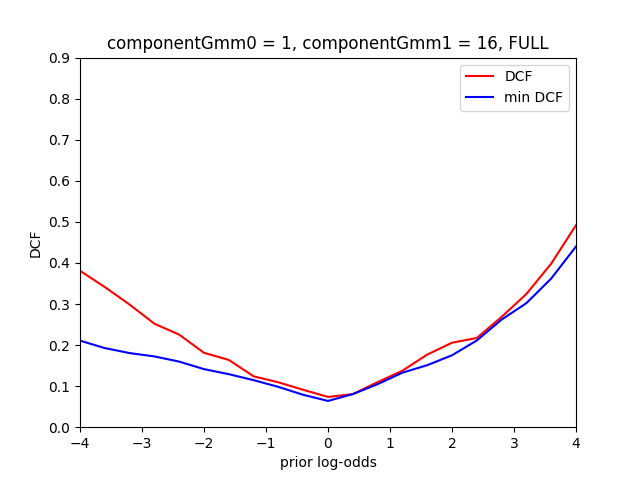
\includegraphics[width=\linewidth]{Lab/10. Lab 10/Images/03. 1-16 Full}
        \label{fig:GMM116Full}
    \end{subfigure}
    \begin{subfigure}[b]{0.23\linewidth}
        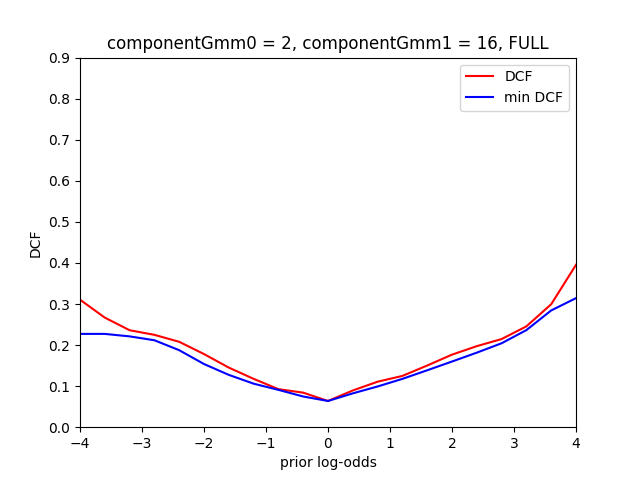
\includegraphics[width=\linewidth]{Lab/10. Lab 10/Images/04. 2 - 16 Full}
        \label{fig:GMM216Full}
    \end{subfigure}
    \begin{subfigure}[b]{0.23\linewidth}
        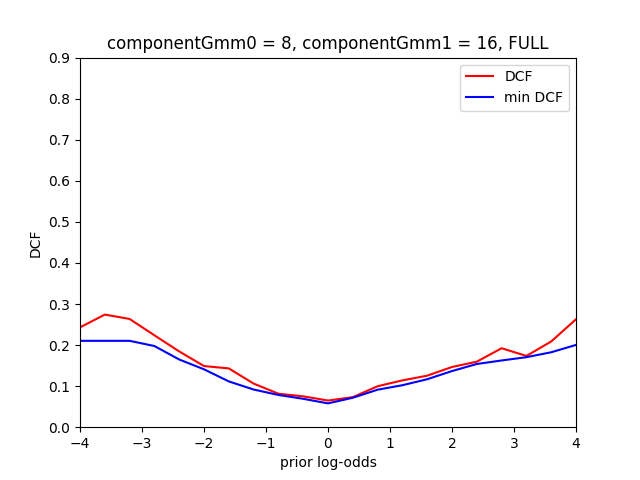
\includegraphics[width=\linewidth]{Lab/10. Lab 10/Images/05. 8-16 Full}
        \label{fig:GMM816Full}
    \end{subfigure}
    \begin{subfigure}[b]{0.23\linewidth}
        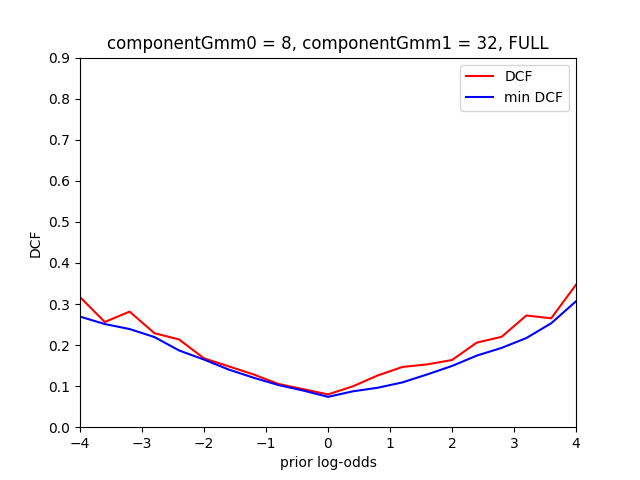
\includegraphics[width=\linewidth]{Lab/10. Lab 10/Images/06. 8 - 32}
        \label{fig:GMM832Full}
    \end{subfigure}
    \caption{Shows minDCF and actDCF for Full Covariance method}
    \label{fig:GMMFullBest}
\end{figure}

\begin{figure}[h!]
    \centering
    \begin{subfigure}[b]{0.23\linewidth}
        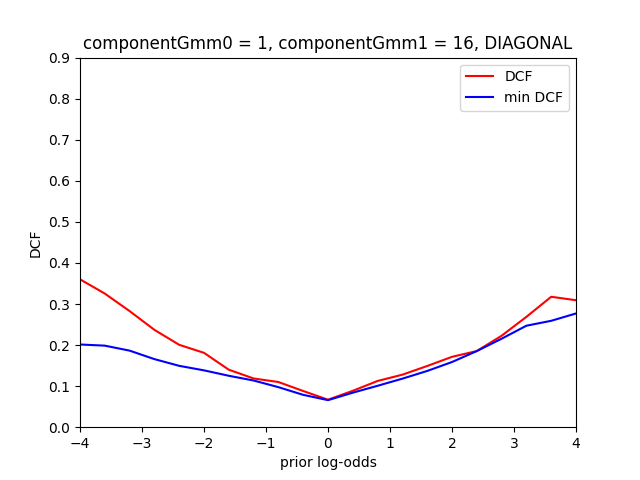
\includegraphics[width=\linewidth]{Lab/10. Lab 10/Images/07. 1-16 Diag}
        \label{fig:GMM116Diag}
    \end{subfigure}
    \begin{subfigure}[b]{0.23\linewidth}
        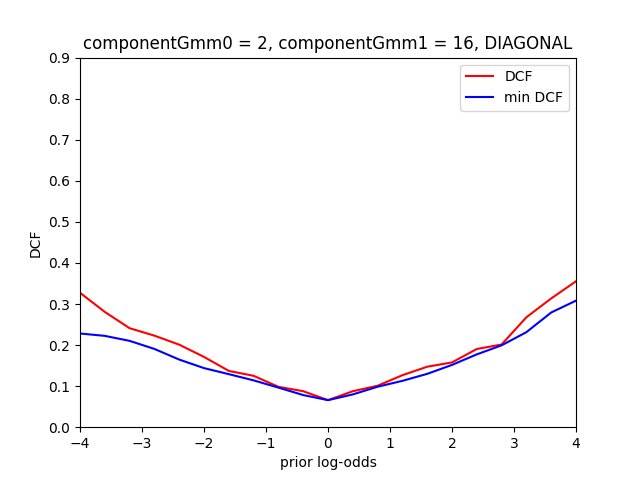
\includegraphics[width=\linewidth]{Lab/10. Lab 10/Images/08. 2-16 Diag}
        \label{fig:GMM216Diag}
    \end{subfigure}
    \begin{subfigure}[b]{0.23\linewidth}
        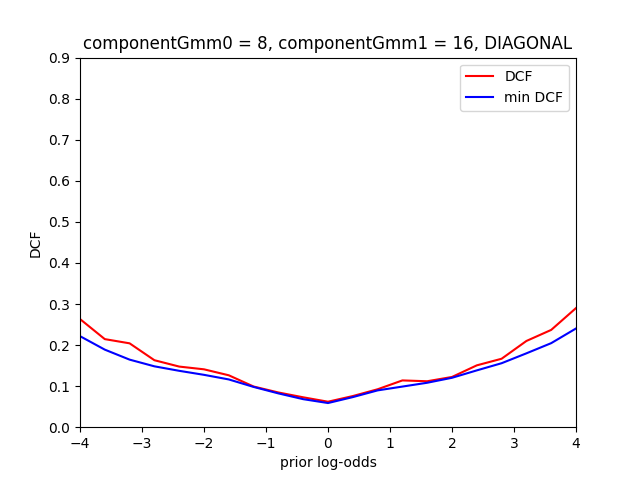
\includegraphics[width=\linewidth]{Lab/10. Lab 10/Images/09. 8-16 Diag}
        \label{fig:GMM816Diag}
    \end{subfigure}
    \begin{subfigure}[b]{0.23\linewidth}
        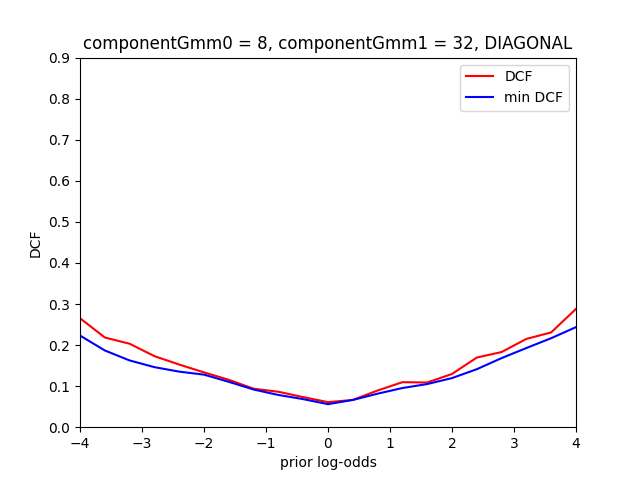
\includegraphics[width=\linewidth]{Lab/10. Lab 10/Images/10. 8-32 Diag}
        \label{fig:GMM832Diag}
    \end{subfigure}
    \caption{Shows minDCF and actDCF for Diagonal Covariance method}
    \label{fig:GMMDiagBest}
\end{figure}

\begin{table}[h!]
    \centering
    \begin{tabular}{>{\centering\arraybackslash}p{2cm} >{\centering\arraybackslash}p{2cm} >{\centering\arraybackslash}p{2cm} >{\centering\arraybackslash}p{2cm} >{\centering\arraybackslash}p{2cm}}
        \toprule
        \multicolumn{5}{c}{\textbf{GMM Model}} \\
        \midrule
        \multirow{2}{*}{\textbf{(nc0, nc1)}} & \multicolumn{2}{c}{\textbf{Full Cov}} & \multicolumn{2}{c}{\textbf{Diag Cov}} \\
        \cmidrule(lr){2-5}
        & \textbf{minDCF} & \textbf{actDCF} & \textbf{minDCF} & \textbf{actDCF} \\
        \midrule
        (1, 16) & 0.1495          & 0.2055          & 0.1433          & 0.1807          \\
        (2, 16) & 0.1701          & 0.1980          & 0.1536          & 0.1731          \\
        (8, 16) & 0.1526          & 0.1725          & 0.1324          & 0.1487          \\
        (8, 32) & 0.1745          & 0.1903          & 0.1312          & 0.1517          \\
        \bottomrule
    \end{tabular}
    \captionsetup{justification=justified,singlelinecheck=false,format=hang}
    \caption{Show minDCF and actDCF for same number of components in GMM}
    \label{tab:GMMBestComponents}
\end{table}

\textbf{Summarize}\par
It can be observed from the results obtained that:
\begin{itemize}
    \item Too high or to low number of components leads to a worsening of the metrics considered.
    \item The best outcomes show that class 0 requires fewer components, meaning it requires a simpler model.
    In contrast, for class 1 it is observed that the number of components is greater this requires a more complex model to avoid underfitting.
    \item Comparing the outcomes with previously applied methods shows that the performance is better but also better calibrated since the gap between minDCF and actDCF is low.
    \item GMM seems to prove to be the best performing model on our data set for several reasons.
    Because the combination of multiple Gaussian distributions allows for better modeling of more complex distributions.
    Also by estimating Gaussian parameters we can effectively model the distributions of the data we have, even if they are complex.
    Finally, through cross-validation we can choose the number of components we think is most correct for each class.
    For all these reasons we can say that in our case this seems to be the model that best fits.
\end{itemize}